%% =============================
%%      IMPORTANTE
%% ESTE ARQUIVO DEVE ESTAR SALVO COMO
%%      UTF - 8
%% =============================

% ----------------------------------------------------------
% Este capítulo é parte integrante do arquivo mestre
% Relatorio_TCC_Mestrado_Base_VERSÃO_SUBVERSÃO
% ----------------------------------------------------------

%==== Novos comandos para escrever nomes pré-formatados
%---
\newcommand{\ufabcFHZ}
{\textbf{\textit{ufabcFHZh.cls}}}
%---
\newcommand{\abntFHZ}
{\textbf{\textit{abntFHZ5.bst}}}
%---
\newcommand{\Fonte}[1]
{{\footnotesize Fonte: #1.}}
%---
\newcommand{\Oautor}
{O autor}
%---
\newcommand{\matlab}
%{Matlab$^\circledR$}
{Matlab\textsuperscript{\textregistered}}
%---
\newcommand{\simulink}
{Simulink\textsuperscript{\textregistered}}
%---
\newcommand{\matlabsimulink}
{Matlab/Simulink\textsuperscript{\textregistered}}
%---
\newcommand{\arduino}
{Arduino\textsuperscript{\textregistered}}
%---
\newcommand{\arduinomega}
{Arduino\textsuperscript{\textregistered} Mega}

%---
\newcommand{\DINAMA}
{\textit{DINAMA}}
%---
\newcommand{\excel}
{Excel\textsuperscript{\textregistered}}
%---
\newcommand{\projetoDaniel}
{\textit{Projeto Daniel}}
%---
\newcommand{\notimpossiblenow}
{\textit{Not Impossible\textsuperscript{Now}}}
%---
\newcommand{\caltech}
{\textit{Caltech}}
%====

% ----------------------------------------- 
% Formas de uso de condicional ifthenelse / toogle para selecionar cores de links
% -----------------------------------------
% http://alvinalexander.com/blog/post/latex/two-simple-examples-using-latex-ifthen-package
% http://tex.stackexchange.com/questions/5894/latex-conditional-expression
% -----------------------------------------
\usepackage{etoolbox} 		% Permite o uso de \newtoggle para criar desvios de fluxo
\usepackage{pdfpages}
%---
\newtoggle{LinksComCores} 	% Opção para selecionar entre links sem cores ou coloridos
% ===
% -----------------------------------------

% ----------------------------------------------------------
% Fim Arquivo
% \usepackage[alf, abnt-emphasize=bf, abnt-thesis-year=both, abnt-repeated-author-omit=no, abnt-last-names=abnt, abnt-etal-cite=3, abnt-etal-list=3, abnt-etal-text=it, abnt-and-type=e, abnt-doi=doi, abnt-url-package=none, abnt-verbatim-entry=no]{abntex2cite}

% Set same dot spacing for list of figures/tables and list of symbols 
%\usepackage{tocbasic}

%\newcommand\Dotfill{\cftdotfill{\cftsecdotsep}}
%   \renewcommand{\cftchapleader}{\cftdotfill{\cftsecdotsep}}


\newcommand{\plotdrs}[4]{ 
\begin{figure}[t]
    \centering
    \begin{subfigure}{0.32\textwidth}
        \centering
        % include second image
        \includegraphics[width=\linewidth]{Figuras/drs/#1/doe_200/drs_#2_all_#3_surface.pdf}  
        \caption{Small dataset.}
        \label{fig:drs_#2_#3_200}
    \end{subfigure}
    \begin{subfigure}{0.32\textwidth}
        \centering
        % include second image
        \includegraphics[width=\linewidth]{Figuras/drs/#1/doe_500/drs_#2_all_#3_surface.pdf}  
        \caption{Medium dataset.}
        \label{fig:drs_#2_#3_500}
    \end{subfigure}
    \begin{subfigure}{0.32\textwidth}
        \centering
        \includegraphics[width=\linewidth]{Figuras/drs/#1/doe_1000/drs_#2_all_#3_surface.pdf}  
        \caption{Large dataset}
        \label{fig:drs_#2_#3_1000}
    \end{subfigure}
    \caption{#4}
    \label{fig:drs_#2_#3}
\end{figure}
}

\newcommand{\plothpoboxplot}[3]{ 
\begin{figure}[t]
    \centering
    \begin{subfigure}{0.3\textwidth}
        \centering
        % include second image
        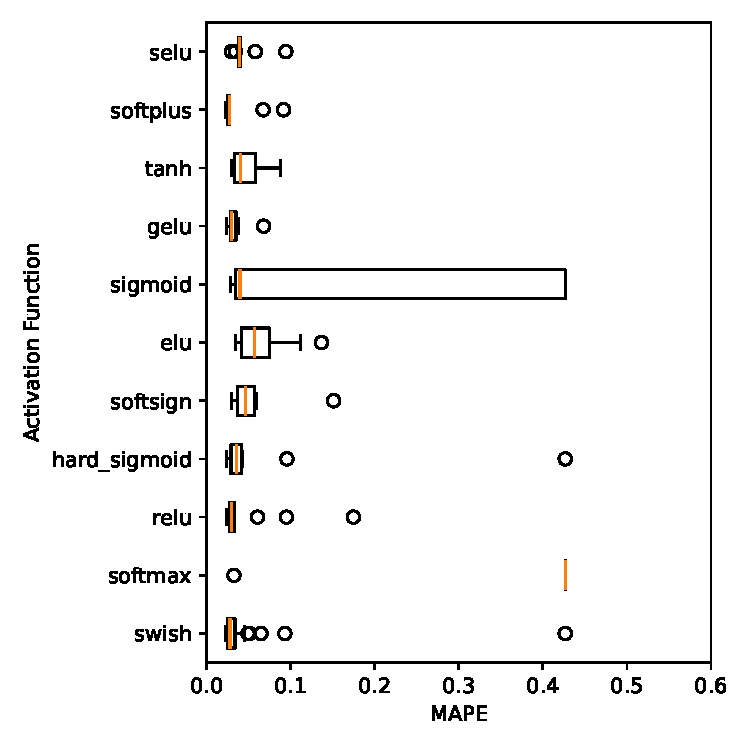
\includegraphics[width=\linewidth]{Figuras/hpo/hpo_plots_#1_#2/hpo_nn_activation_MAPE.pdf}  
        \caption{MAPE.}
        \label{fig:hpo_MAPE_a#1_#2}
    \end{subfigure}
    \begin{subfigure}{0.3\textwidth}
        \centering
        % include second image
        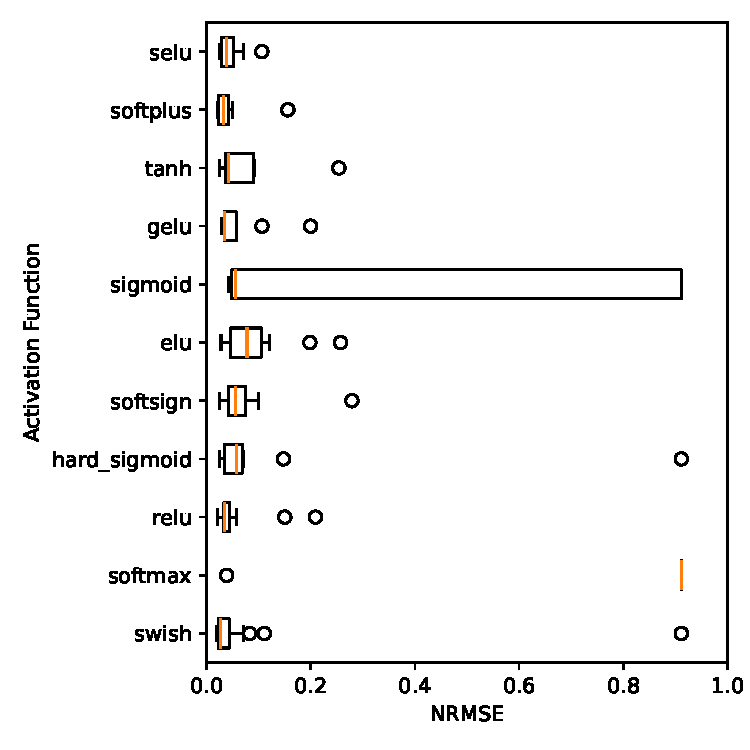
\includegraphics[width=\linewidth]{Figuras/hpo/hpo_plots_#1_#2/hpo_nn_activation_NRMSE.pdf}  
        \caption{NRMSE.}
        \label{fig:hpo_NRMSE_#1_#2}
    \end{subfigure}
    \begin{subfigure}{0.3\textwidth}
        \centering
        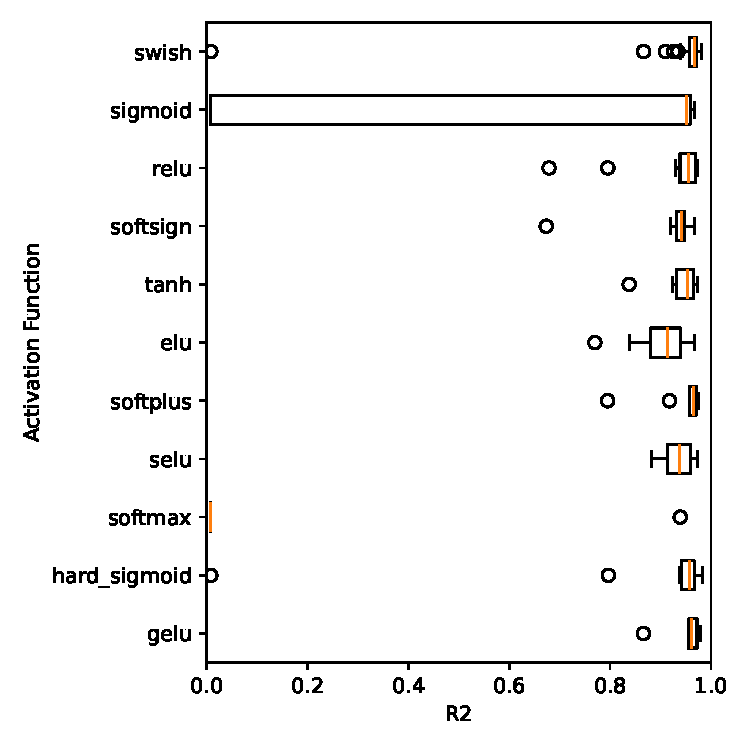
\includegraphics[width=\linewidth]{Figuras/hpo/hpo_plots_#1_#2/hpo_nn_activation_R2.pdf}  
        \caption{R2}
        \label{fig:hpo_R2_#1_#2}
    \end{subfigure}
    \caption{#3}
    \label{fig:hpo_#1_#2}
\end{figure}
}

\newcommand{\plothpomap}[3]{
\begin{figure}[t]
    \centering
    \begin{subfigure}{0.3\textwidth}
        \centering
        % include second image
        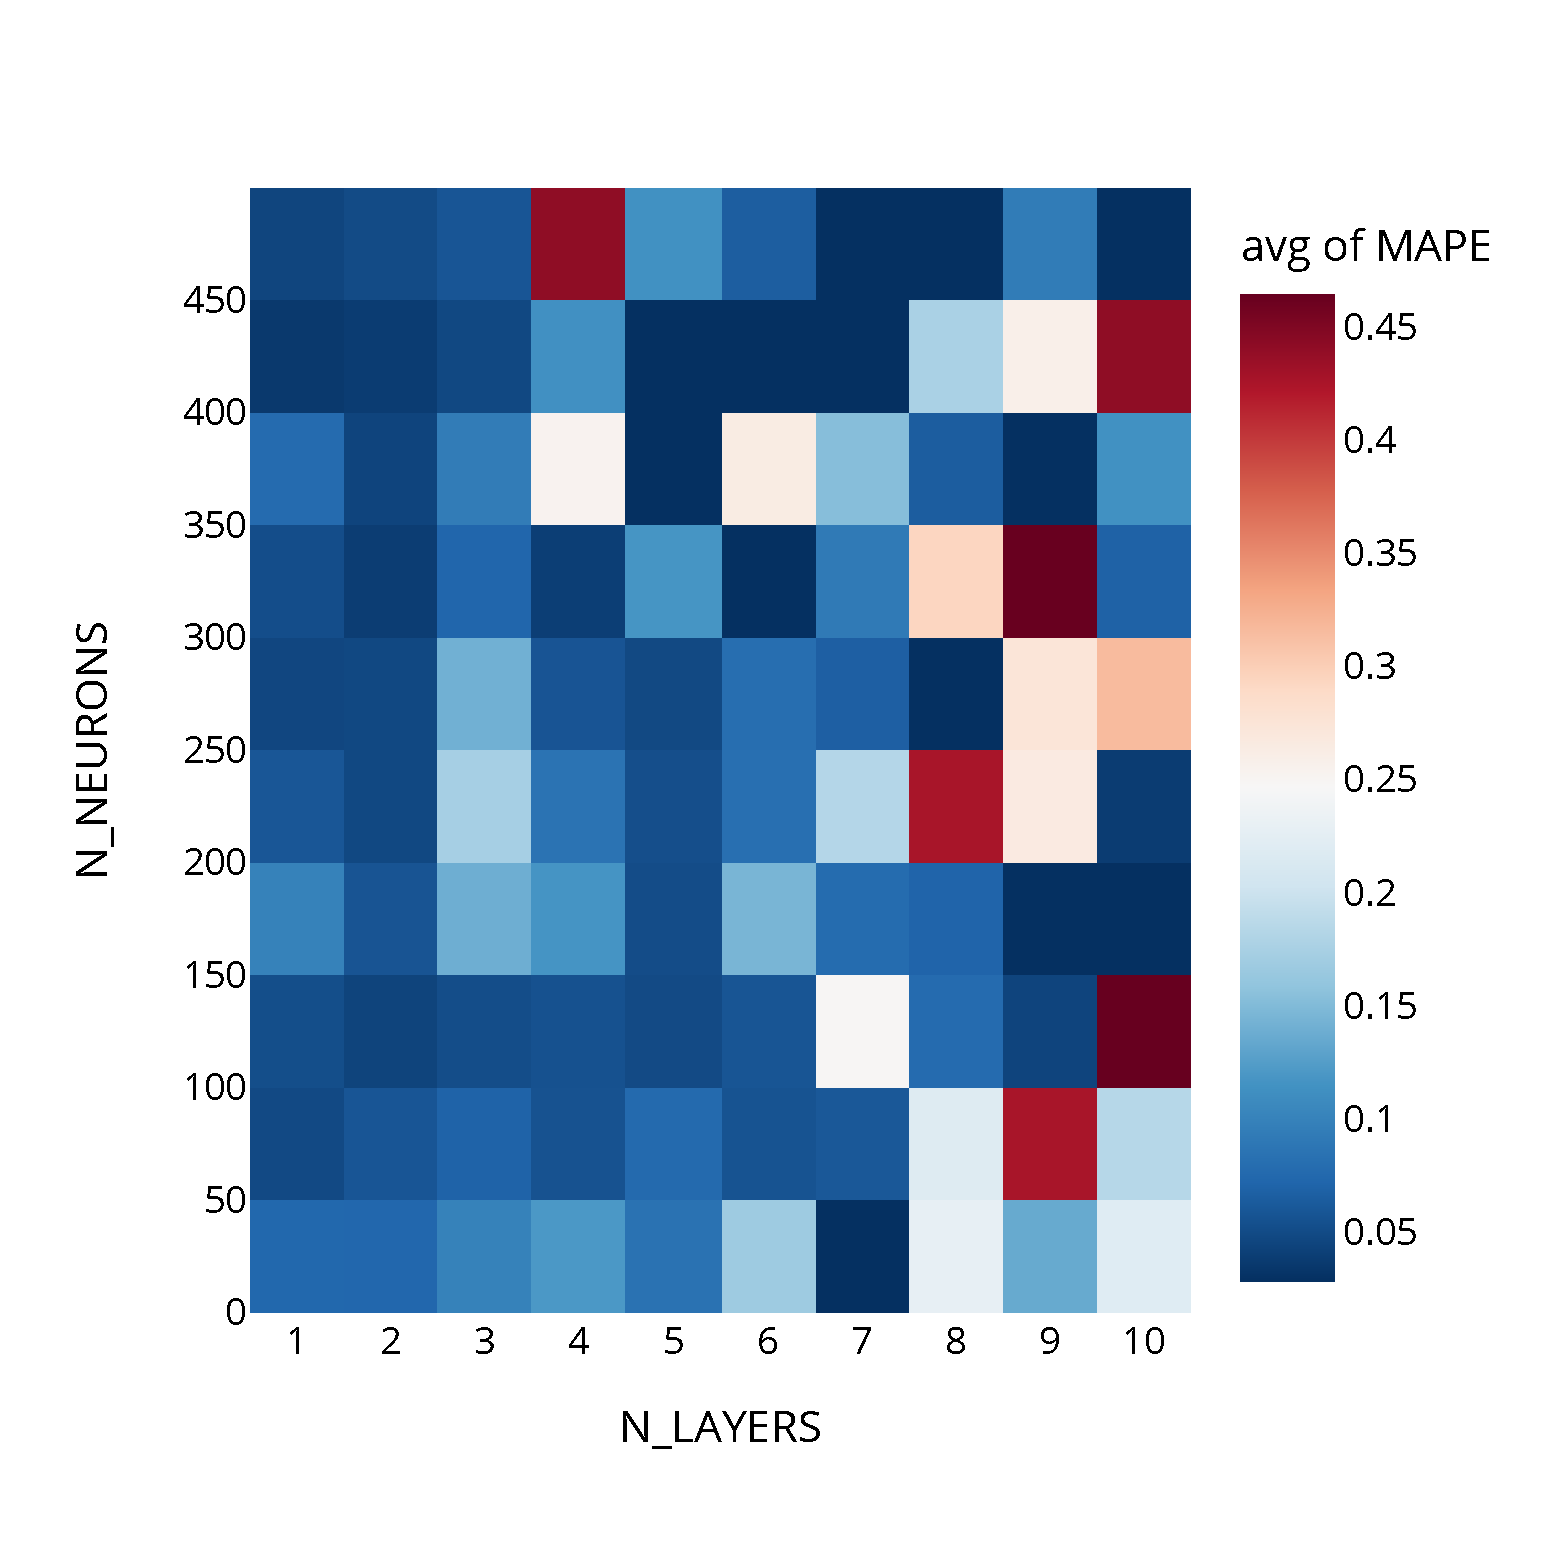
\includegraphics[width=\linewidth]{Figuras/hpo/hpo_plots_#1_#2/neurons_layers_heat_map_MAPE.pdf}  
        \caption{MAPE.}
        \label{fig:hpo_map_MAPE_all_all}
    \end{subfigure}
    \begin{subfigure}{0.3\textwidth}
        \centering
        % include second image
        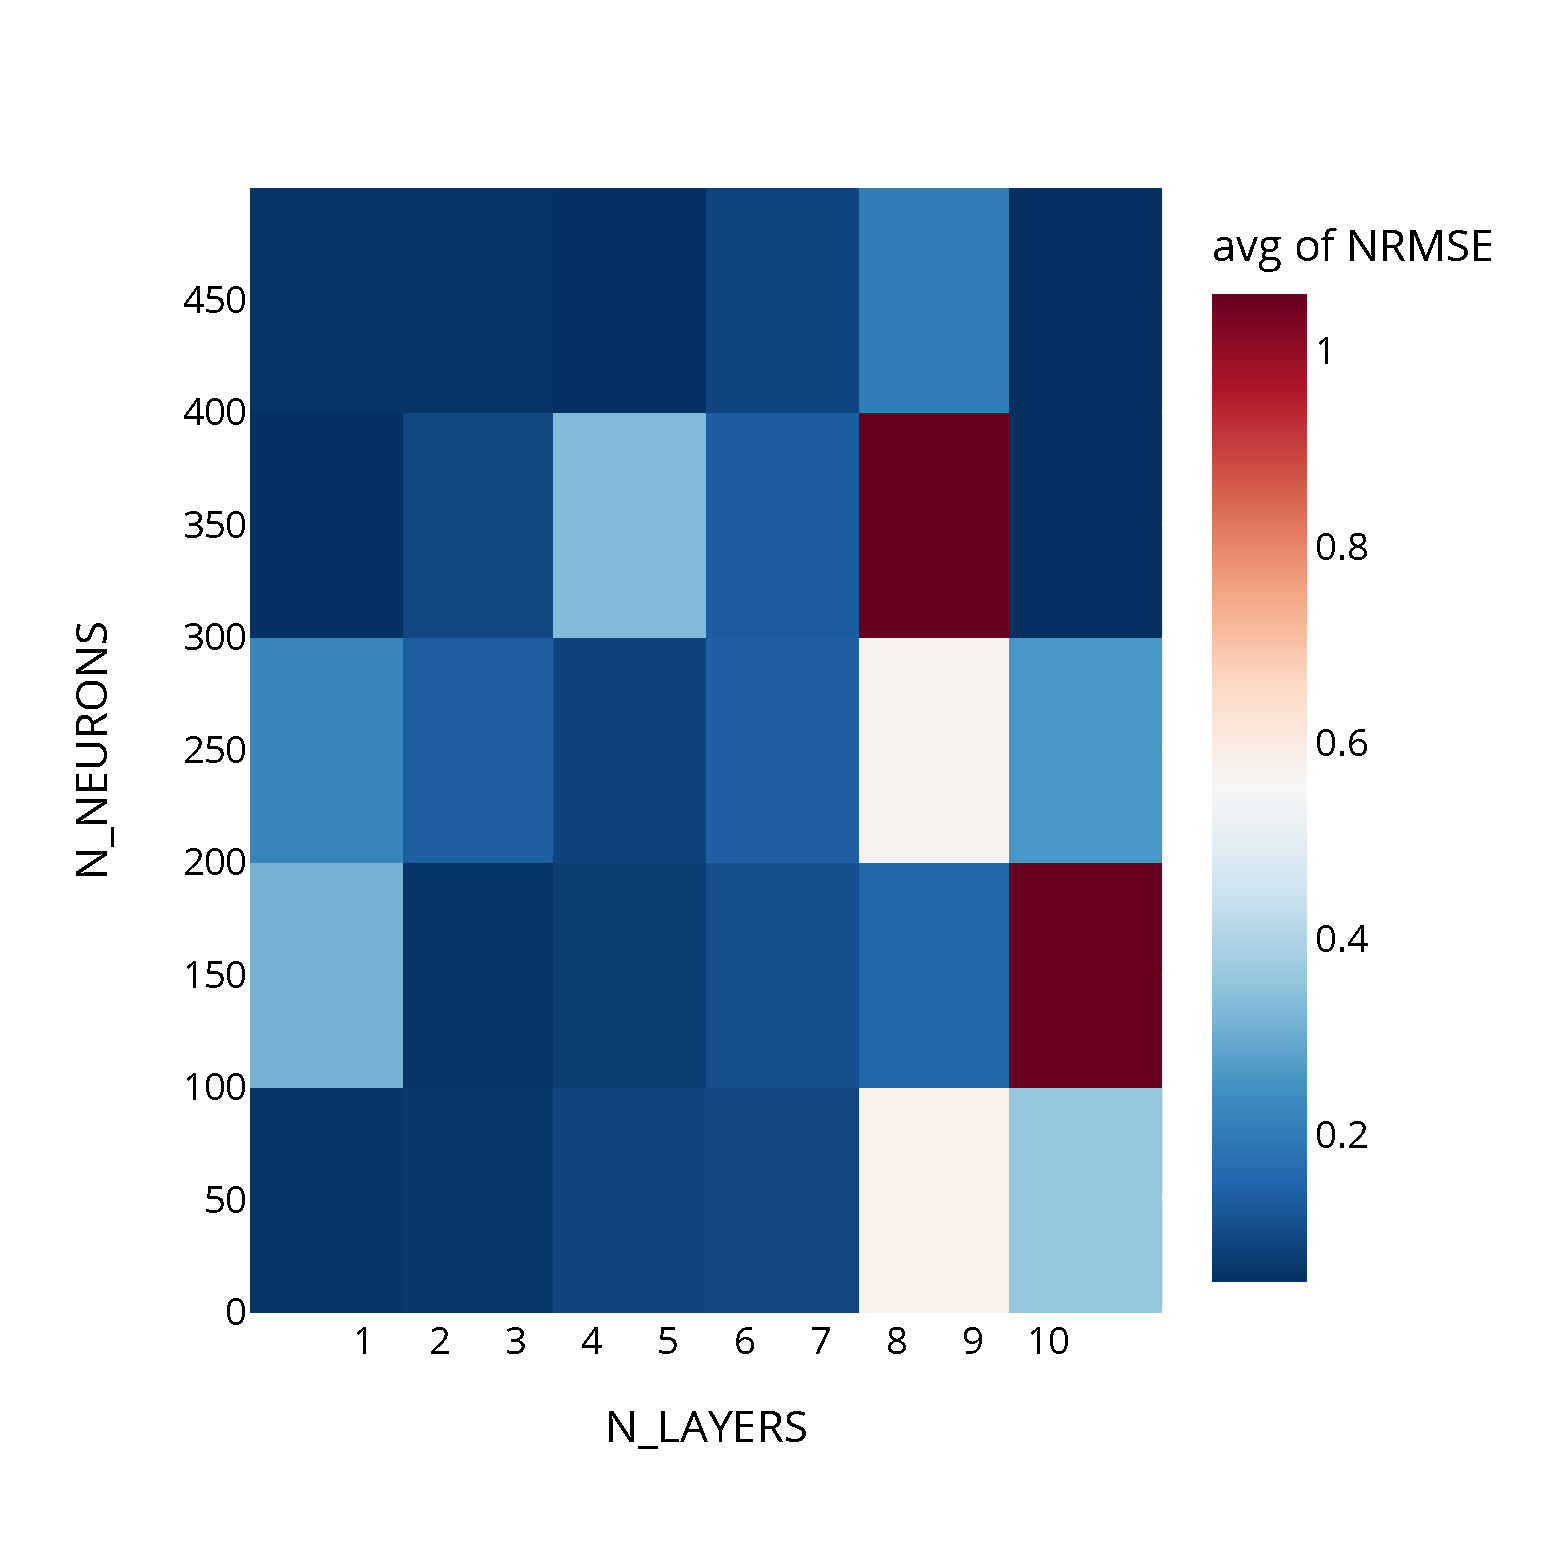
\includegraphics[width=\linewidth]{Figuras/hpo/hpo_plots_#1_#2/neurons_layers_heat_map_NRMSE.pdf}  
        \caption{NRMSE.}
        \label{fig:hpo_map_NRMSE_all_all}
    \end{subfigure}
    \begin{subfigure}{0.3\textwidth}
        \centering
        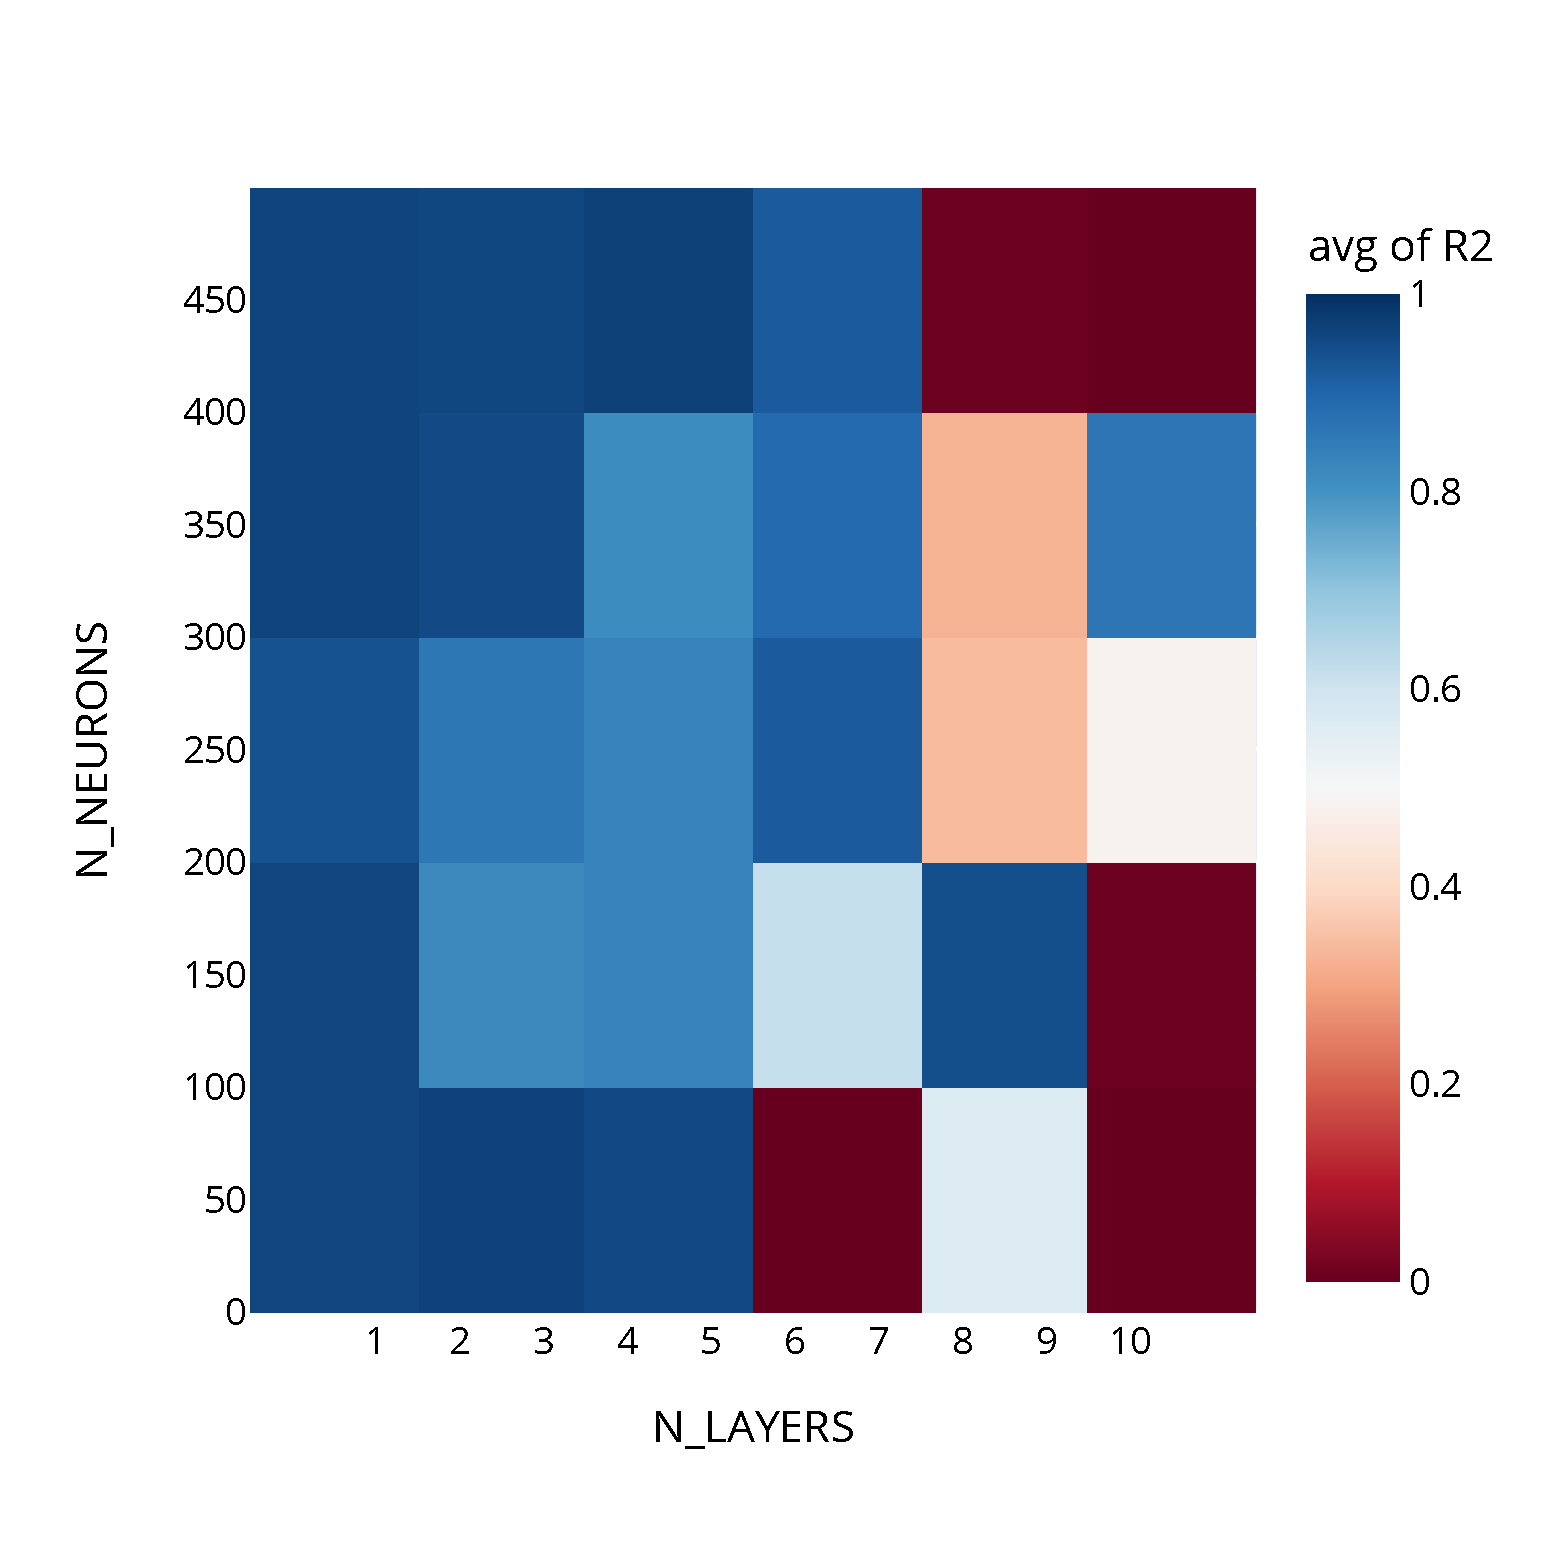
\includegraphics[width=\linewidth]{Figuras/hpo/hpo_plots_#1_#2/neurons_layers_heat_map_R2.pdf}  
        \caption{R2}
        \label{fig:hpo_map_R2_all_all}
    \end{subfigure}
    \caption{#3}
    \label{fig:hpo_map_all_all}
\end{figure}
}

\newcommand{\plothpohistogram}[3]{
\begin{figure}[t]
    \centering
    \begin{subfigure}{0.3\textwidth}
        \centering
        % include second image
        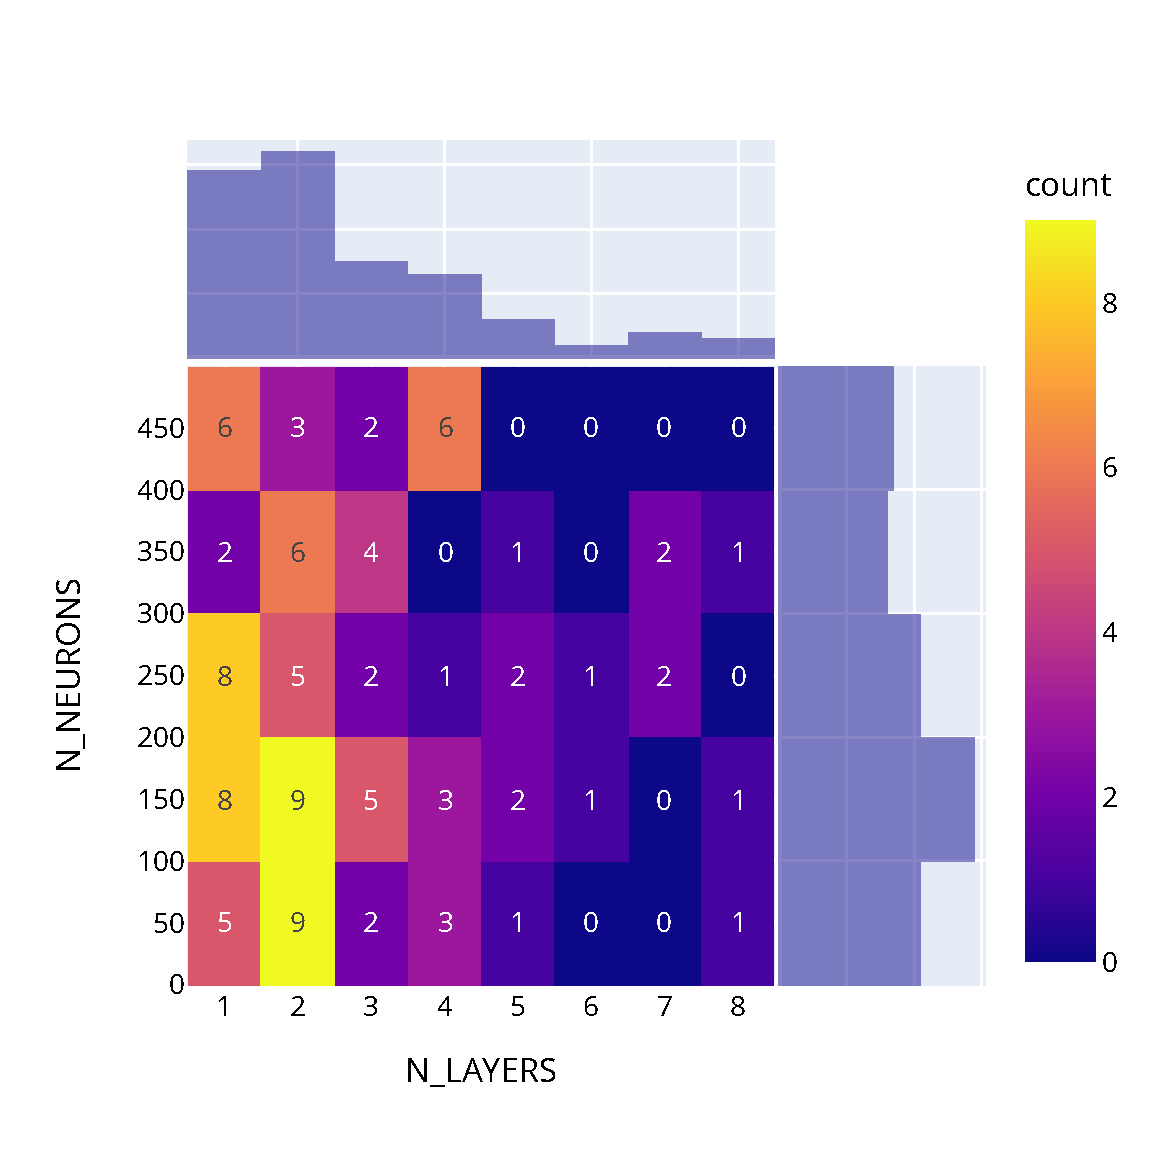
\includegraphics[width=\linewidth]{Figuras/hpo/hpo_plots_#1_#2/hpo_nn_hist_neurons_layers.pdf}  
        \caption{Histogram neurons layers.}
        \label{fig:hpo_hist_neurons_#1_#2}
    \end{subfigure}
    \begin{subfigure}{0.3\textwidth}
        \centering
        % include second image
        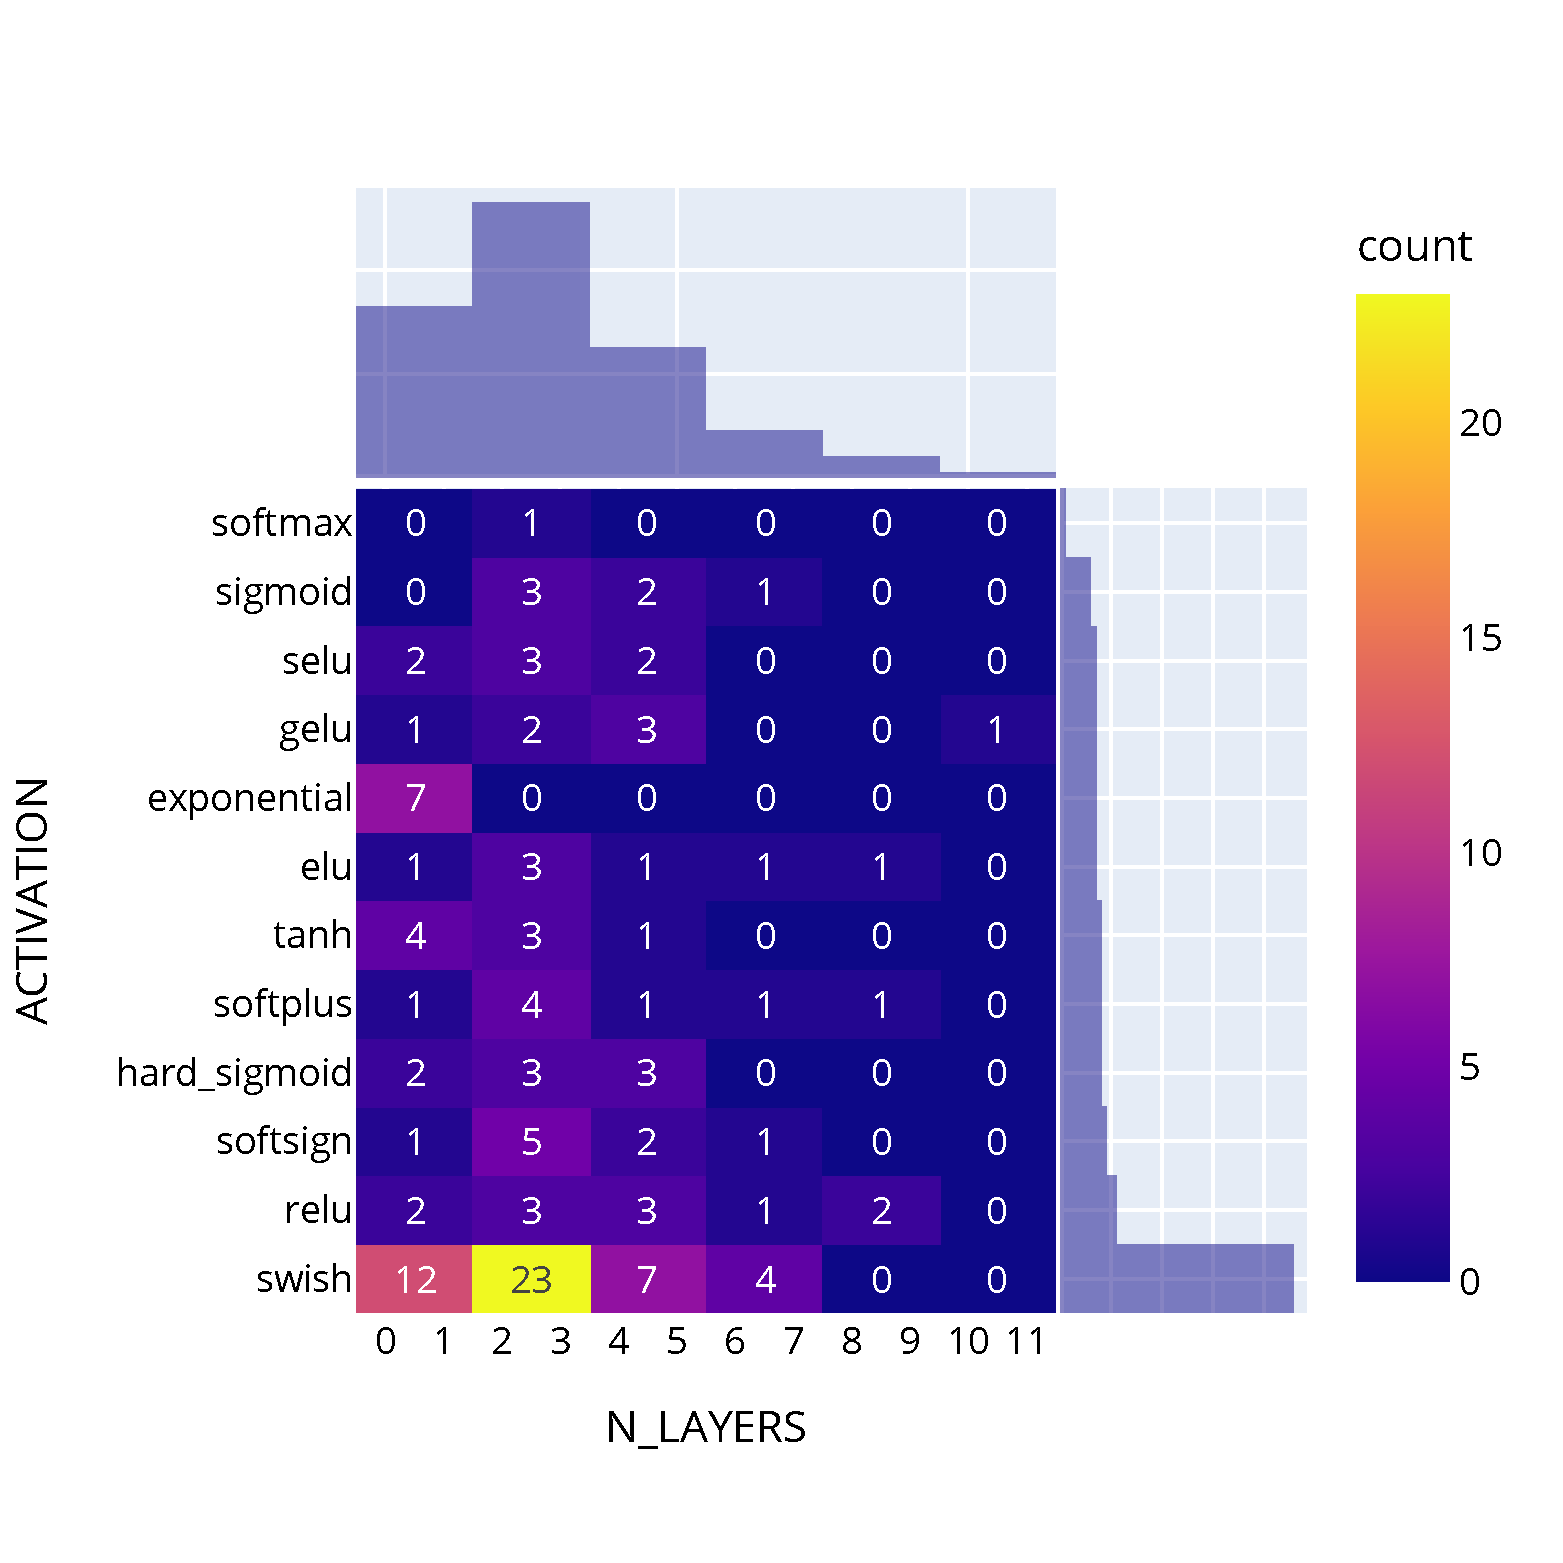
\includegraphics[width=\linewidth]{Figuras/hpo/hpo_plots_#1_#2/hpo_nn_activation_layers_count.pdf}  
        \caption{Histogram activation layers.}
        \label{fig:hpo_hist_activation_#1_#2}
    \end{subfigure}
    \begin{subfigure}{0.3\textwidth}
        \centering
        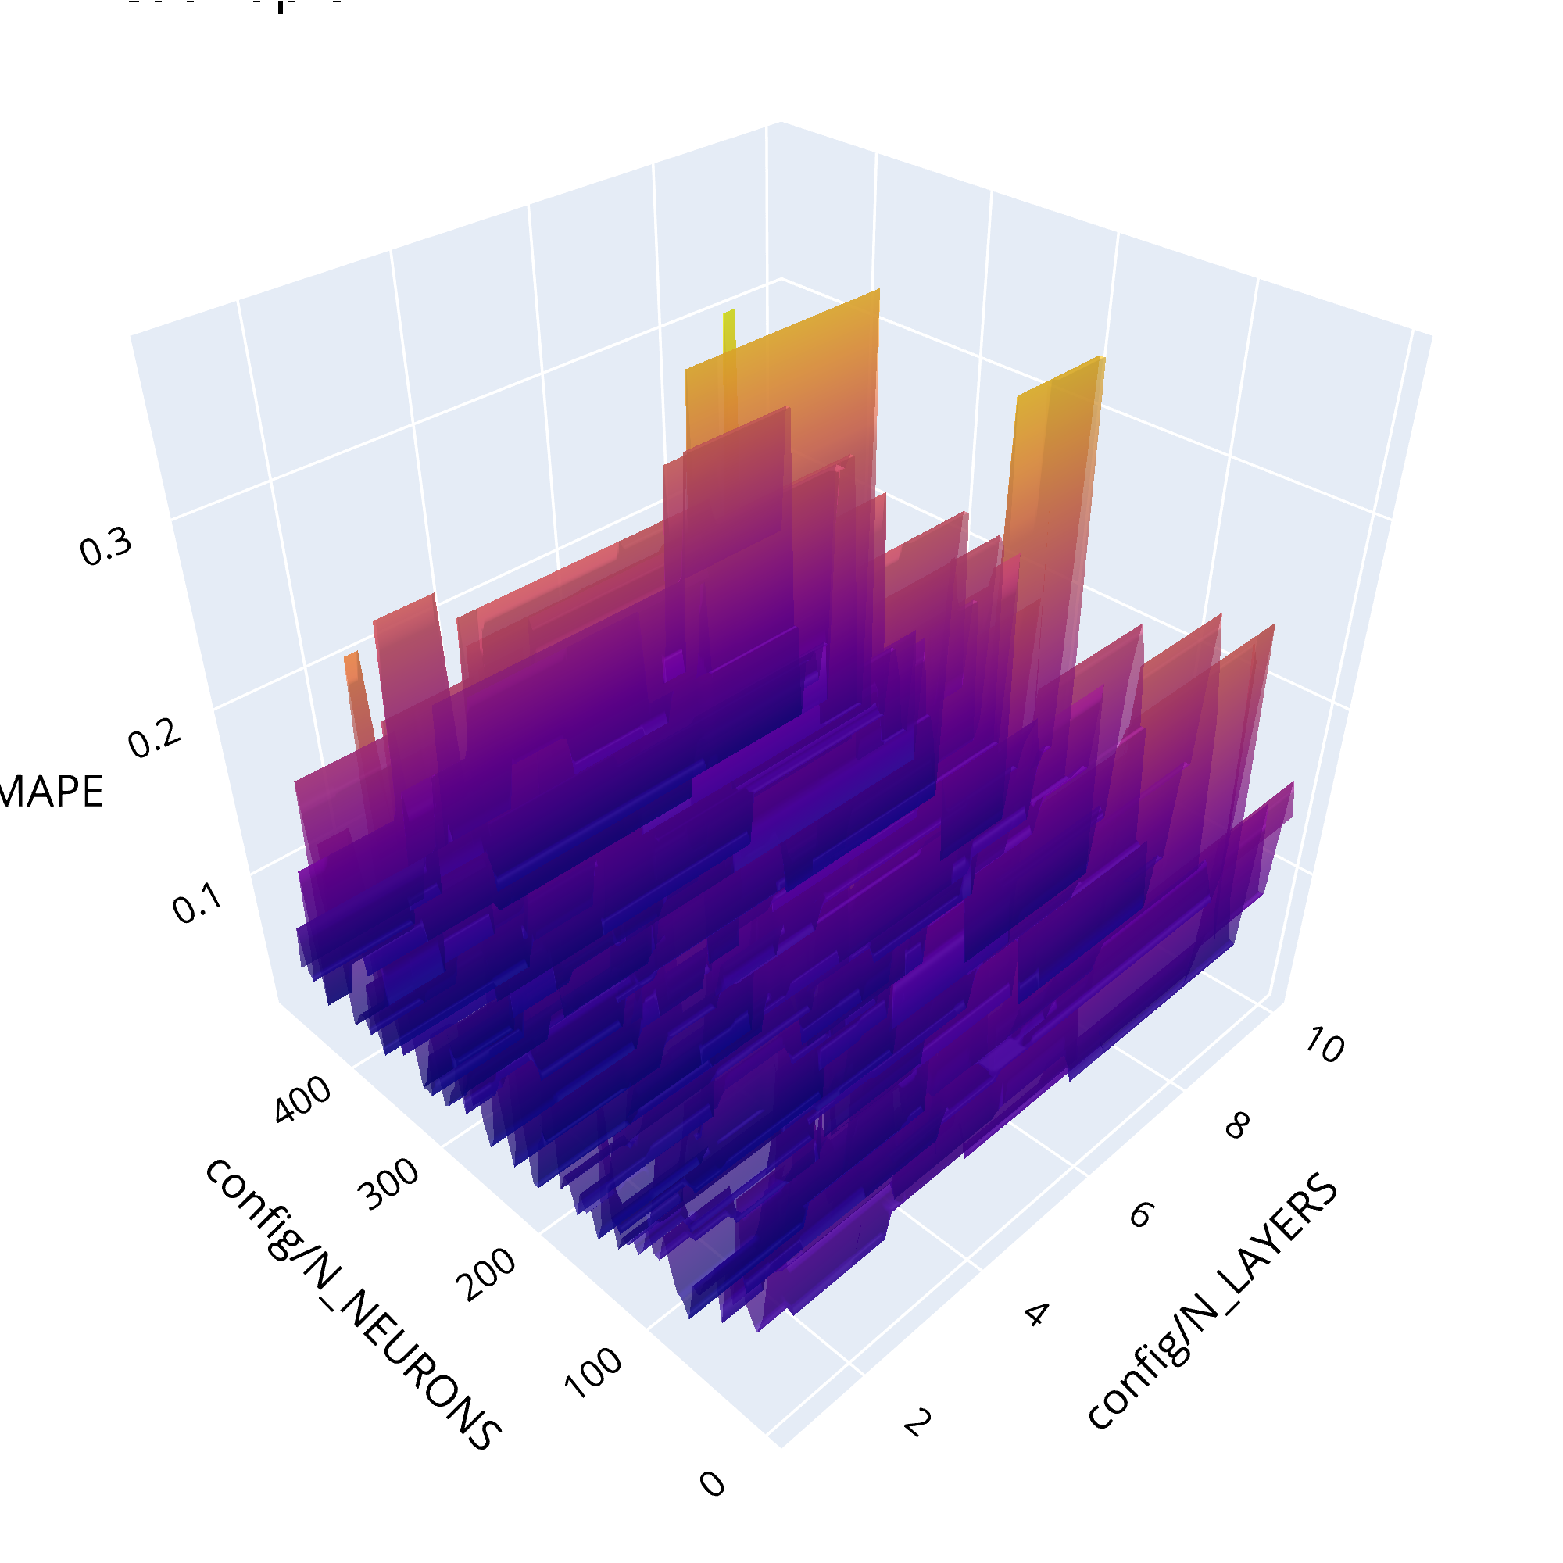
\includegraphics[width=\linewidth]{Figuras/hpo/hpo_plots_#1_#2/hpo_nn_activation_layers_surface.pdf}  
        \caption{Surface MAPE}
        \label{fig:hpo_surface_MAPE_#1_#2}
    \end{subfigure}
    \caption{#3}
    \label{fig:hpo_hist_#1_#2}
\end{figure}
}